\chapter{Controlling Laplacian Eigenfluids}
Many real world applications require us to optimize for some parameters of
a physics-based problem. A toy example would be to optimize for some initial
angle and velocity of a projectile to hit some target \todo{Refer back to the
learning to throw example}. As a more involved example, \cite{MinDrag} address
finding the best shape to minimize drag. These kinds of inverse problems have
been around for quite some time in engineering applications.

Building on all of the previous ideas, we now introduce our investigation into
the use of eigenfluids in fluid control problems, making use of their explicit
closed form description of a velocity field (\todo{link to equation}) to derive
gradients used for optimization. Our main proposition is to achieve
reduced-order modeling-like speed increase: in lieu of representing the fluid on
a grid, we reconstruct the velocity field only at discrete points in space,
while simulating the dynamics of the fluid in a reduced dimensional
space.\todo{Link to eq.}

In the following, we showcase different optimization scenarios, where we try out
different aspects of controlling eigenfluids via \acf{DP} gradients. (See
section~\ref{dp-loss}.)

We start with examples of "traditional" optimization scenarios. By
"traditional", we mean finding individual solutions to problems via some
optimization technique -- in our case, \acf{GD}. Moving further, we look for
generalized solutions to a set of problems by training \acfp{NN}.

We implemented all of our experiments using $\Phi_{Flow}$
(\cite{holl2019pdecontrol}).

\section{Matching Velocities}\label{section:matching-velocities}
To verify the feasibility of our technique before moving on to more involved
setups, our most straightforward optimization scenario is finding an initial
basis coefficient vector $\vb{w}_0 \in \mathbb{R}^N$ for an eigenfluid
simulation using $N=16$ basis fields, such that when simulated for $t$ time
steps, the reconstructed $\mathcal{R}\vb{w}_t = \vb{u}_t$ velocity
field will match some precalculated $\vb{u}^*: [0,\pi]\times[0,\pi] \to
\mathbb{R}^2$ target velocity field:

\begin{equation}\label{eq:match-vel-loss}
  L(\vb{w}) = \left|
  \mathcal{R}\mathcal{P}^{t}(\vb{w}) - \vb{u}^*
  \right|_2^2,
\end{equation}

where $\mathcal{P}^t(\vb{w}) = \mathcal{P} \circ \mathcal{P} \dots \circ
\mathcal{P}(\vb{w})$ is the physical simulation of base coefficients $\vb{w}$
(in the reduced dimension) $t$ times.

For the optimization, we initialize a $\vb{w}_\text{init} \in \mathbb{R}^N$
vector with random numbers (from a normal/Gaussian distribution), and run the
eigenfluid simulation for $t$ timesteps, after which, we measure the error as
given by loss function \eqref{eq:match-vel-loss}. Relying on backpropagation to
derive the necessary gradients, we use the \ac{GD} optimization method as
introduced in equations~\eqref{eq:gd-steps} to iteratively find a vector
$\vb{w}_{optim}$, yielding a low scalar loss $L(\vb{w}_{optim})$.

To be able to make some further evaluation of the end results possible, we step
an eigenfluid solver for time $t$ to precalculate the target $\vb{u}^*$ velocity
field, sampled on a $32\times32$ grid. We denote the initial base coefficient
vector of this reference simulation $\vb{w}^*$, but keep in mind that the
optimization has absolutely zero knowledge of this value, as it sees only the
$32\times32\times2$ velocity values of $\vb{u}^*$ at time $t$. Also, these
values could have been precalculated from any other kind of fluid simulation as
well, or even just initialized randomly. Deriving $\vb{u}^*$ as the result of an
eigenfluid simulation has the added benefit of exposing to us a solution
$\vb{w}^*$ that we can use to compare with the solution of the optimizer.

We test this setup on two scenarios, with differing the number of timesteps
simulated: first with $t=16$, and then with $t=100$.

For $t=16$ simulation steps, starting from a loss of around $400$, the first
$100$ \ac{GD} optimization steps with $\lambda=10^{-3}$ reduced the loss to
under $1.0$, while $200$ steps further decreased it to under $4*10^{-4}$, with
each further step still continuously decreasing the error. 

Naturally, this very basic method has its limits.  Optimizing for initial
coefficients based solely on that when reconstructed on a $32\times32$ grid
after $100$ steps of a non-linear simulation, they should match a given velocity
field, proved to be a substantially harder problem, as even a relatively small
error can accumulate into major deviations over these longer timesteps,
resulting in much less stable gradients. With using the same learning rate, the
optimization diverged almost instantly. With some tuning of the learning rate
$\lambda$ in the range of $[10^{-4}, 10^{-8}]$, we were able to get the loss
below $0.14$.  (Starting from an initial loss of $320$ from the random
initialization.) 

We visualize the results of these two scenarios in
Figure~\ref{fig:matching-velocities}. It is interesting to observe that even
though the optimization had absolutely no knowledge of $\vb{w}^*$, only
a comparison with a precomputed $\vb{u^*}$ velocity field at timestep $100$, the
optimized $\vb{w}_{optim}$ vector already starts to look similar to $\vb{w}^*$.
Keep in mind that this is not guaranteed at all, as highlighted with the
\todo{link to learning to throw example}. In some other cases of running this
optimization setup, we also observed $\vb{w}_{optim}$s that are completely
different from $\vb{w}^*$. Due to the physical constraints of the eigenfluids
simulation, in these cases the optimization could not change any of the $16$
values of $\vb{w}_{optim}$ locally in a way that would further reduce the loss
below some small number, and was stuck in a local minima of the parameter space.

Although there are a number of ways to tweak this setup, we can already verify
from these results that  the flow of the gradients is working, and is ready to
be tested in more advanced scenarios.

\begin{figure}
  \centering
  \begin{subfigure}{\textwidth}
    \centering
    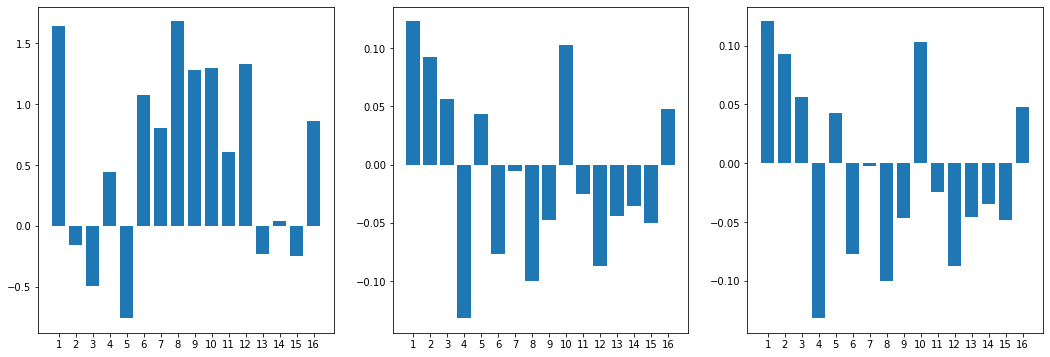
\includegraphics[width=0.9\textwidth]{figures/finding-initial-velocities/t_16_coefficients.png}
    \caption{$\vb{w}_{init}$, $\vb{w}_{optim}$, and
    $\vb{w}^*$, optimizing for velocity field after $16$ timesteps}
    \label{fig:16-timesteps-coeffs}
  \end{subfigure}\par\medskip
  \begin{subfigure}{\textwidth}
    \centering
    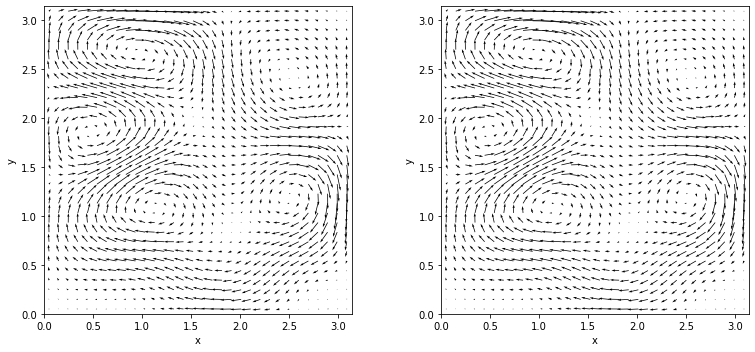
\includegraphics[width=0.8\textwidth]{figures/finding-initial-velocities/t_16_velocities.png}
    \caption{Target $\vb{u}^*$, and $\vb{u}^{16}$, reconstructed from
      $\mathcal{P}^{16}(\vb{w}_{optim})$\\}
    \label{fig:16-timesteps-vel}
  \end{subfigure}\par\medskip
  \begin{subfigure}{\textwidth}
    \centering
    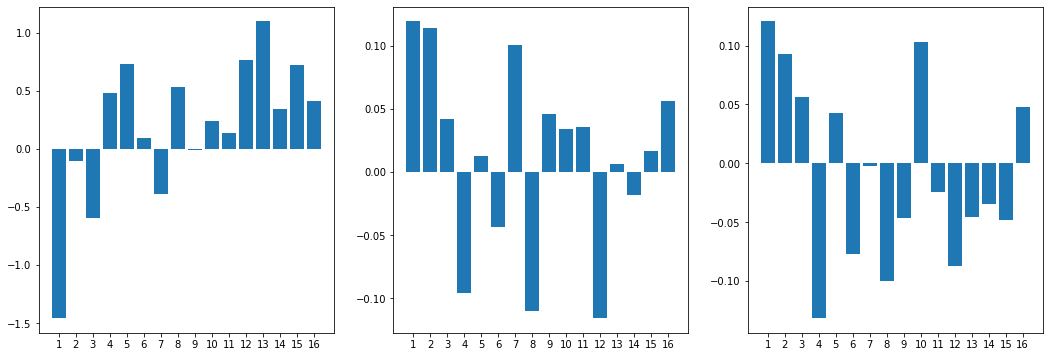
\includegraphics[width=0.9\textwidth]{figures/finding-initial-velocities/t_100_coefficients.png}
    \caption{Initial basis coefficients $\vb{w}_{init}$, $\vb{w}_{optim}$, and
    $\vb{w}^*$, optimizing for velocity field after $100$ timesteps\\}
    \label{fig:100-timesteps-coeffs}
  \end{subfigure}\par\medskip
  \begin{subfigure}{\textwidth}
    \centering
    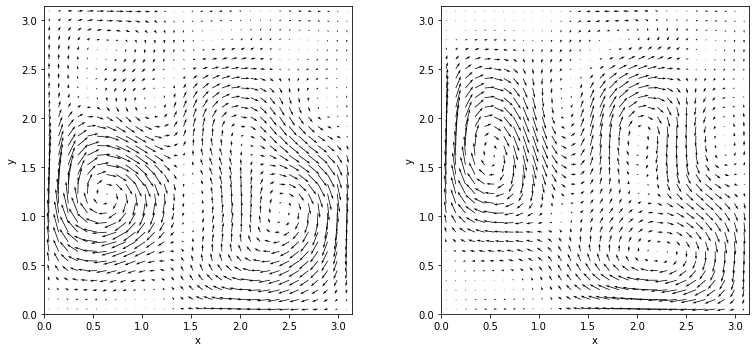
\includegraphics[width=0.8\textwidth]{figures/finding-initial-velocities/t_100_velocities.png}
    \caption{Target $\vb{u}^*$, and $\vb{u}^{100}$, reconstructed from
      $\mathcal{P}^{100}(\vb{w}_{optim})$}
    \label{fig:100-timesteps-vel}
  \end{subfigure}
  \caption{Results of optimizing for an initial $\vb{w}_0$ basis coefficient
    vector that matches a target velocity field $\vb{u}^*$ when reconstructed
    after simulating for $t$ timesteps.
  }
  \label{fig:matching-velocities}
\end{figure}

\section{Controlling Shape Transitions}
\label{section:controlling-shape-transitions}
In the following, we showcase an optimization scenario, with the target of
controlling the transition between two marker shapes in a fluid simulation
setup. 
\footnote{Note that we use the terms \textit{smoke}, \textit{marker},
\textit{density}, and \textit{scalar valued density/marker function}
interchangeably throughout the text.}
The work of \cite{holl2019pdecontrol} formulated this problem in an
Eulerian representation, with explicitly simulating the shapes as scalar marker
densities being advected by the velocity field of the simulated fluid. 

Playing to the strength of the eigenfluids method, our method makes use of
an explicit formulation of the fluid velocity $\vb{u}$ as described in
section~\todo{ref section}. We stay independent of a grid resolution, and
approximate the 2D shapes via a set of sample points. We reconstruct the
velocity field only partially at these discrete points as needed for the
advection of these particles. This results in both a faster fluid simulation as
well as optimization as compared to fully simulating an $N\times N$ grid,
advecting a marker density, and backpropagating gradients of a physical
simulation with much more degrees of freedom.

We formulate three different control problems, each with a different mean to
exert control over the fluid simulation.
\begin{itemize}
  \item First, in a similar vein to the problem statement in
    section~\ref{section:matching-velocities}, we are looking for an initial
    coefficient vector $\vb{w}_0$ of an eigenfluids simulation, such that when
    simulated for $t$ time steps, the reconstructed velocity field advects some
    initial points to the desired positions.
  \item Second, we optimize for some force vector $\vb{f}\in \mathbb{R}^{t\times
    N}$, such that $\vb{f}_t \in \mathbb{R}^N$ applied as external force to each
    timestep of an eigenfluid simulation, it yields the desired outcome.
  \item Finally, we generalize the problem to looking for a function that exerts
    the necessary control force at time $t$, such that particles currently at
    positions $\vb{p}_t$ end up at target positions $\vb{p}_{t+1}$ at the
    next timestep. We formulate this third task as a \acf{NN} agent in the
    form $\vb{f}(\vb{p_t}, \vb{p_{t+1}}, \vb{w}_{t}, \boldsymbol\theta)$, also
    passing in the current basis coefficient vector $\vb{w}_t$, and optimizing
    for its parameters $\boldsymbol\theta$ to yield the desired outcome.
\end{itemize}

In each of these tasks, a velocity field $\vb{u} = \mathcal{R}\vb{w}$ advects
a set of initial points $\vb{p}_0 = \left[\vb{p}_0^0,\dots, \vb{p}_0^i\right]$
to line up with target positions $\vb{p}_t = \left[\vb{p}_t^0, \dots,
\vb{p}_t^i\right]$.  We formulate this as 

\begin{equation}
  L(\vb{w}, \vb{p}_0, \vb{p}_t)
  = \left| \mathcal{P}^{t}(\vb{p}_0, \vb{w}) - \vb{p}_t\right|_2^2 
  = \sum_{i}\left|\mathcal{P}^{t}(p_0^i, \vb{w}) - p_t^i\right|_2^2, 
\end{equation}

where $\mathcal{P}^t(\vb{w}, \vb{p}) = \underbrace{\mathcal{P} \circ
\mathcal{P}\circ \dots \circ \mathcal{P}(\vb{w}, \vb{p})}_{t \text{ times}}$
denotes the physical simulation of base coefficients $\vb{w}$ and points
$\vb{p}$ in $\vb{u} = \mathcal{R}\vb{w}$, the velocity field reconstructed from
$\vb{w}$.  We use a simple mean-square error (also known as squared $L_2$ norm)
for measuring the error.

\subsection*{Sampling}
Advection of some scalar quantity in a fluid is an abstract problem that
describes many real-world phenomena. We can think of the transport of some ink
dropped into water, clouds in the air, or some buoyant smoke rising. Phenomena
such as these can be modeled as a density function $\psi(\vb{x})$ defined over
the simulation domain $D$. In a fluid with velocity $\vb{u}$, and $\div{\vb{u}}
= 0$ (i.e. the fluid is incompressible), the advection is governed by the
equation

$$\pdv{\psi}{t} + \vb{u}\cdot \grad{\psi} = 0.$$

In Eulerian fluid simulation methods as described by \cite{StableFluids}, both
$\vb{u}$ and $\vb{\psi}$ are sampled on grids, numerically approximating the
evolution of the field quantities. Instead, our method proposes sampling the
density function at discrete particle positions, thus rephrasing the process in
a Lagrangian way.

In the context of Laplacian eigenfluids, a Lagrangian viewpoint is especially
inviting, as the explicit description of the fluid velocity $\vb{u}$ \todo{Refer
to equation} allows us to reconstruct $\vb{u}$ only partially, while keeping the
simulation of the fluid dynamics in a reduced dimensional space. In a forward
physics simulation, this can already lead to substantial speed-ups, but this
formulation seems especially promising when the backpropagation of variables is
desired, such as the optimization scenarios introduced herein.

A straightforward way to define a shape is
\begin{equation}\label{eq:binary-shape-function}
\psi(\vb{x}) = 
\begin{cases}
  1, & \qq*{inside the shape}\\
  0, & \text{outside the shape}.\\
\end{cases}
\end{equation}
Sampled on an $N \times N$ grid, this is equivalent to a binary image with
a resolution of $N \times N$. Moreover, when sampled on a grid, and advected,
it is straightforward to interpret the resulting grid and its values as
a grayscale image with values $[0,\dots,1]$.

Often used in 3D scanning, reconstruction and scene understanding problems,
a \acf{SDF} can be defined as the distance to the surface (in 2D, the edge) of
an object, with positive values outside, and negative values inside. In our
implementation, we define our shapes as \acp{SDF}. For example, a circle with
radius $r$ and center $\vb{o} = (o_x, o_y)^T$ is defined as

$$\text{SDF}_{\text{circle}}(\vb{x, \vb{o}, r}) 
  = \abs{\vb{x}-\vb{o}} - r
  = \sqrt{(x-o_x)^2 + (y-o_y^2)} - r.$$

For simulating (and visualizing) the advection dynamics of these shapes, we
transform the SDFs to a binary form as in
equation~\eqref{eq:binary-shape-function}.

As we neither want to lose too much information about our original function, nor
want to keep track of an unnecessary number of points, the feasibility of this
method necessitates an efficient sampling of $\psi(\vb{x})$. We use a simple
rejection-based sampling technique. Transforming the shapes to fit inside the
unit rectangle $[0,1]\times[0,1]$, we generate random points
$\vb{p}_\text{sample}\in [0,1]\times[0,1]$, rejecting them if they lie outside
the shape.

As we consider shape transitions given start and target shapes $S_\text{0}$ and
$S_\text{t}$, it is important to take into consideration the connection between
these shapes. To balance finding spatial correspondences between the shapes,
while still approximating their unique shapes, we sample $O$ overlapping, and
$U$ unique points. For the overlapping points, we accept only
$\vb{p}_\text{sample} \in S_\text{0} \cup S_\text{t}$, i.e. we reject points
that are not inside both shapes (transforming both shapes to fit inside the unit
square for the sampling). For the unique points we sample a different set of
points for each shape. 

To generate low-discrepancy, quasi-random 2D coordinates, we use a Halton
sequence (\cite{halton}), giving deterministic coordinates, given coprimes $p$
and $q$. Using one set of primes for sampling $O$ overlapping points, and
another set of primes for sampling $U$ unique points can give us further
overlapping points, as the proposed (but potentially rejected) sequence of
points will be the same for both shapes.

We further generate $T=5$ trivial points that are hand-picked to best resemble
the given shape, as well as line up between different shapes. We choose these to
be the center, upper right, upper left, lower left, and lower right corners of
the shape. 

In conclusion, our final set of $\vb{p}_0$ initial, and $\vb{p}_t$ target sample
positions are given by concatenating the $O$ overlapping, $U$ unique, and $T$
trivial points for each shape, resulting in two set of sample points $\vb{p}_0,
\vb{p}_t \in \mathbb{R}^{O+U+T}$.

Figure~\ref{fig:sampling} shows the result of our sampling strategy for
a triangle and a circle shape.

\begin{figure}
  \centering
  \begin{subfigure}[t]{0.48\textwidth}
    \centering
    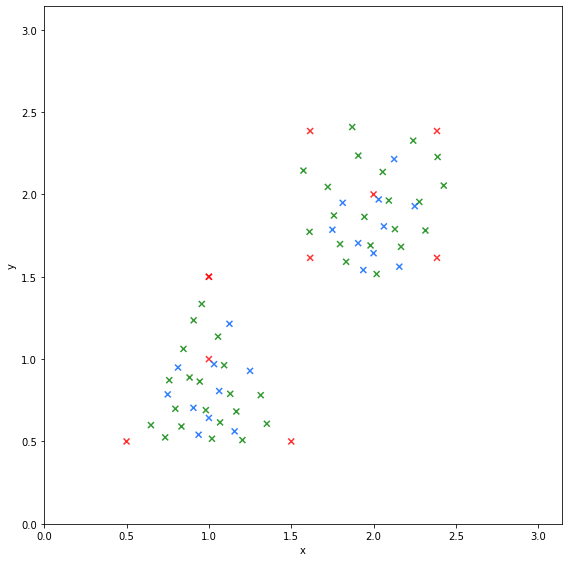
\includegraphics[width=\textwidth]{figures/sampling/points.png}
    \caption{The $O=30$ overlapping (blue), $U=30$ unique (green), and $T=5$
    trivial (red) points for each shape.}
  \end{subfigure}
  \begin{subfigure}[t]{0.48\textwidth}
    \centering
    % 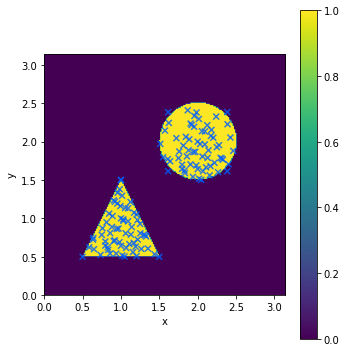
\includegraphics[width=\textwidth]{figures/sampling/smokes.png}
    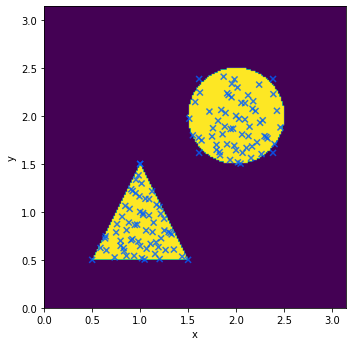
\includegraphics[width=\textwidth]{figures/sampling/smokes_no_bar.png}
    \caption{Sample points plotted over $\psi_\text{triangle}
    + \psi_\text{circle}$.}
  \end{subfigure}\par\medskip
  \caption{Sampling strategy for transitioning from a triangle to a circle.
  Halton series with base $(2,7)$ and $(3,11)$ were used to generate the
  overlapping and unique positions, respectively.}
  \label{fig:sampling}
\end{figure}

\todo{Would it make sense to write any of these as an Algorithm? (Maybe in
a parallel universe, haha.)}

\subsection{Initial Velocity}

\todo{Finish this section}
$$
\arg\min_{\vb{w}} \left| \mathcal{P}^{t}(\vb{p}^0, \vb{w})
  - \vb{p}^t\right|_2^2
  $$
Making use of the differentiability of our physical simulator $\mathcal{P}$, and
the multivariable chain rule for deriving the gradient of the above
$\mathcal{P}^t$ function composition, we can derive its gradient with respect to
the initial coefficients: $$\frac{\partial
\mathcal{P}^t(\vb{w},\vb{p})}{\partial \vb{w}}.$$

Finally, we simply iterate a \ac{GD} optimizer with learning rate $\lambda$ to
find a (good enough) solution for our above minimization problem:

$$\vb{w}_{\text{better}} = \vb{w} - \lambda
\frac{
    \partial\text{Loss}(\vb{w}, \vb{p}_0, \vb{p}_t)
}{
    \partial \vb{w}
}$$

The main difficulty of this non-linear optimization problem lies in that we have
no control over the natural flow of the fluid besides supplying an initial
$\vb{w}_0$ vector.

\subsection{Control Force Estimation}
In this scenario, we are optimizing for a force vector $\vb{f} \in
\mathbb{R}^{t\times N}$, such that $\vb{f}_t \in \mathbb{R}^N$ applied as
external force to each timestep of an eigenfluid, some initial positions
$\vb{p}_0$ will be advected to target positions $\vb{p}_t$ after $t$ timesteps:

$$\arg\min_{\vb{f}} \left| \mathcal{P}^{t}(\vb{p}_0, \vb{w}, \vb{})
  - \vb{p}_t\right|_2^2$$

\begin{figure}
  \centering
  \begin{subfigure}{\textwidth}
    \centering
    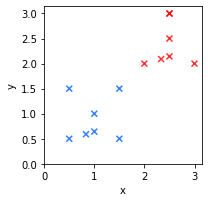
\includegraphics[width=0.3\textwidth]{figures/f-optim/blue_start_red_target.png}
    \caption{Initial (blue), and target (red) sample points.}
  \end{subfigure}\\
  \begin{subfigure}{\textwidth}
    \centering
    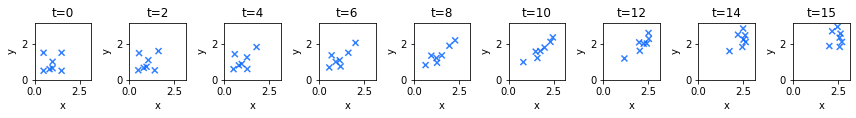
\includegraphics[width=\textwidth]{figures/f-optim/trajectory_horizontal.png}
    \caption{Optimized trajectory of the sample points.}
  \end{subfigure}\par\medskip
  \begin{subfigure}{\textwidth}
    \centering
    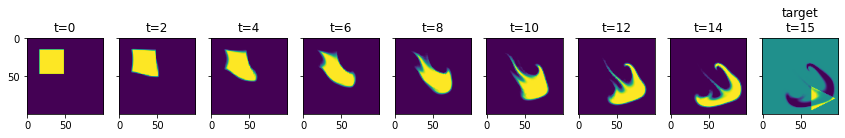
\includegraphics[width=\textwidth]{figures/f-optim/smoke_trajectory_horizontal.png}
    \caption{Smoke advection for qualitative comparison, reconstructed on
    a $100\times 100$ grid.}
  \end{subfigure}\par\medskip
  \caption{Force optimization results.}
  \label{fig:f_optim}
\end{figure}

\subsection{Neural Network Training}
\todo{Write about fully connected architecture...}

\subsection*{Overfitting to a single training sample}
We overfit the \ac{NN} to a single training sample. We plot the results of
the time evolution on figure~\ref{fig:NN-overfit}. We observe that a reduced
degress of freedom can yield comparable, or even better results with the same
setup, and training time. 

\begin{figure}
  \centering
  \begin{subfigure}{\textwidth}
    \centering
    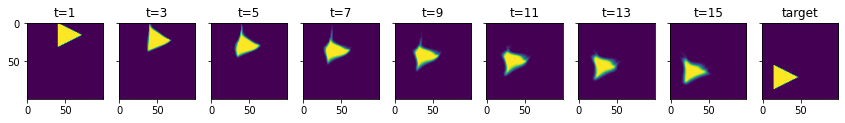
\includegraphics[width=\textwidth]{figures/nn-training/NN_N16_triangle_overfit_horizontal.png}
    \caption{$N=16$ basis fields}
  \end{subfigure}
  \begin{subfigure}{\textwidth}
    \centering
    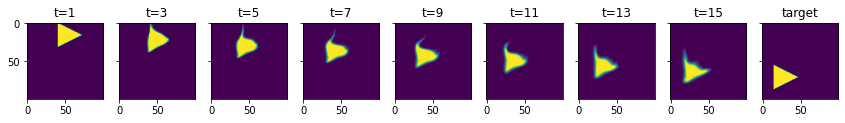
\includegraphics[width=\textwidth]{figures/nn-training/NN_N36_triangle_overfit_horizontal.png}
    \caption{$N=36$ basis fields}
  \end{subfigure}
  \caption{Time evolution of simulating two overfitted \ac{CFE} \acp{NN} to
  a single shape transition for $16$ timesteps $t=[0\dots15]$. Using $O=30$
overlapping, $U=40$ unique, and $T=5$  trivial sample points.}
  \label{fig:NN-overfit}
\end{figure}

\subsection*{Training}
We generate $2000$ samples, using $1800$ for training, and $200$ for validation.
Using $N=16$ basis fields, we train a \ac{NN} for the same \ac{CFE} problem as
detailed above. 

We generate further data the \ac{NN} has not seen during training to further
test generalization. 

\begin{figure}
  \centering
  \begin{subfigure}{\textwidth}
    \centering
    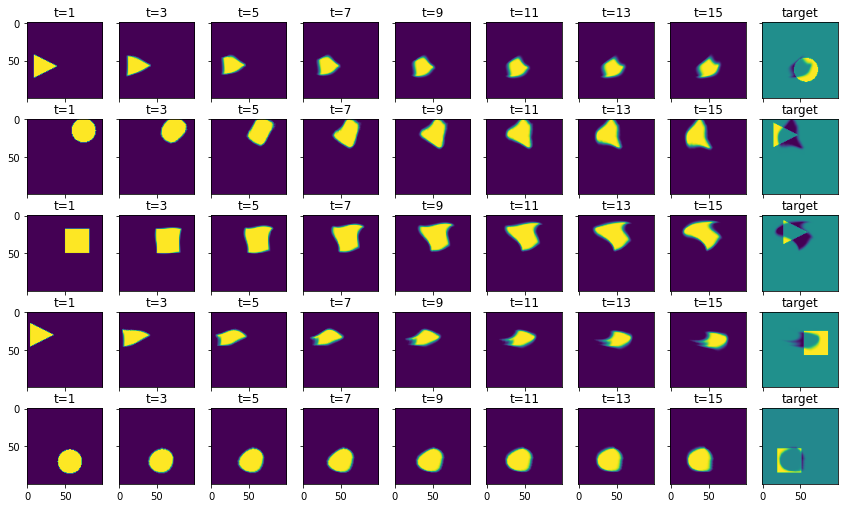
\includegraphics[width=\textwidth]{figures/nn-final/trained_trajectories_horizontal.png}
    \caption{Randomly sampled trajectories from the \textbf{training} data.}
  \end{subfigure}
  \begin{subfigure}{\textwidth}
    \centering
    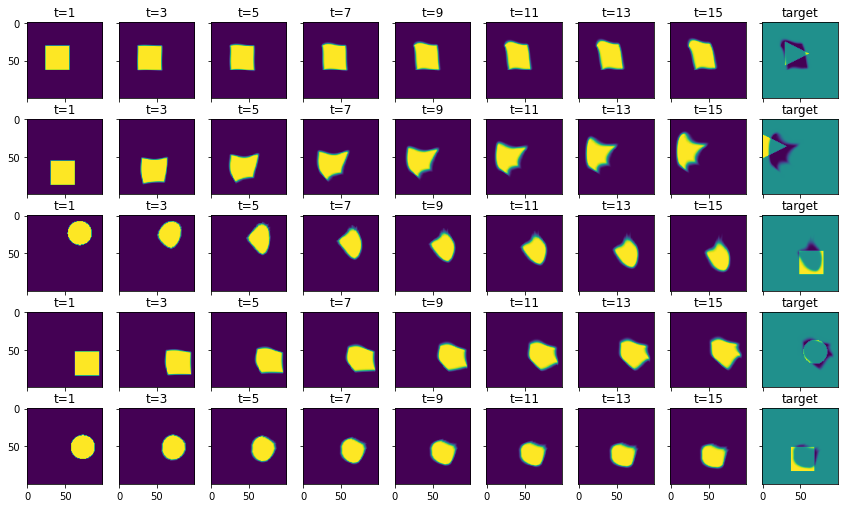
\includegraphics[width=\textwidth]{figures/nn-final/test_trajectories_horizontal.png}
    \caption{Randomly sampled trajectories from the previously unseen, randomly
    generated \textbf{test} set.}
  \end{subfigure}
  \caption{Randomly sampled time evolution of controlled shape transition
  tasks. Using $N=16$ basis fields, sampling the smokes on a $32\times 32$ grid,
  approximating them with $O=30$ overlapping, $U=40$ unique and $T=5$ trivial
  sample points, through $16$ timesteps $t=[0\dots15]$.}
  \label{fig:NN-shape-transition}
\end{figure}
